\documentclass{beamer}
\usepackage{tikz,framed}
\usetikzlibrary{arrows,positioning,decorations.pathmorphing}
\setbeamertemplate{navigation symbols}{}

\title{EE 382N Lecture 10}
\author{Lecturer: Vijay Garg \\ Scribe: Sameer Bibikar}
\date{September 29, 2020}

\begin{document}
\begin{frame}
\titlepage
\end{frame}

\begin{frame}{Detecting Unstable Predicates}
\begin{itemize}
\item If $B$ is a stable predicate, then $\textrm{possibly} : B$
and $\textrm{definitely} : B$ are basically the same!

\item But for unstable predicates this becomes more complicated.

\item Last time, we showed that $\textrm{possibly} : B$ is
$NP$-complete for general $B$.

\item Can we use global snapshots instead?
\end{itemize}
\end{frame}

\begin{frame}{Lattice-Linear Predicates: an example}
    \begin{itemize}
        \item Simple example: \emph{conjunctive predicates} are linear:
        
        $$B \equiv \ell_1 \wedge \ell_2 \wedge \dots \wedge \ell_n,$$
        
        where $\ell_i$ is a local predicate to process $i$.
        \item If $B$ is false, then there exists some $i$ for which
        $\ell_i$ is false, and the predicate can be true only by
        advancing process $i$.
    \end{itemize}
\end{frame}

\begin{frame}{Forbidden States}
    \begin{itemize}
        \item Definition (forbidden state). Given any predicate $B$,
        $i$ is \emph{forbidden} in $G$ if
        
        $$\mathrm{forbidden}(G, i) \equiv \forall H : G \le H,
        (G[i] \ne H[i]) \vee \neg B(H).$$
        \item In other words, leaving process $i$ in the same state
        will guarantee that the predicate can't become true.
    \end{itemize}
\end{frame}

\begin{frame}{Lattice-Linear Predicates}
\begin{itemize}
    \item Definition (lattice-linear predicate). A predicate $B$ is
    \emph{lattice-linear} iff
    
    $$\forall G : \neg B(G) \implies \exists i : \mathrm{forbidden}(G, i).$$
    
    \item If $\neg B(G)$, then without advancing process $i$, it is
    impossible to make $B$ true.
\end{itemize}
    
\end{frame}

\begin{frame}{Lattice-Linear Predicates: examples}
    \begin{itemize}
        \item conjunctive predicates
        \item stable matching problem
        \item shortest path problem (what is the minimum value needed
        to reach some other point?)
        \item market clearing prices ($n$ bidders, items with
        different prices. Can we assign items to bidders?)
    \end{itemize}
\end{frame}

\begin{frame}{Example of non-lattice-linear predicate}
\begin{columns}[T]
\begin{column}[t]{0.48\linewidth}
\begin{itemize}
    \item Consider $B \equiv x + y \ge 1$.
    \item Look at the orange global state where $\neg B$.
    \item Neither local state is forbidden: we can escape
    the condition that $\neg B$ by simply advancing the
    \emph{other} process.
    \item Thus $B$ is not lattice-linear.
\end{itemize}
\end{column}
\begin{column}{0.48\linewidth}
    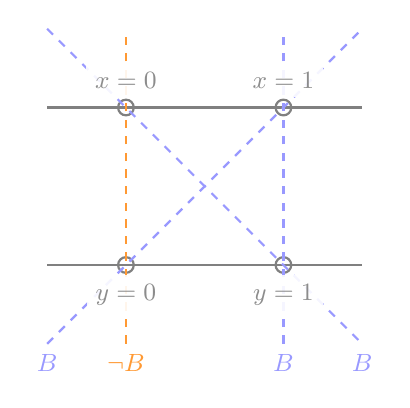
\begin{tikzpicture}[event/.style={circle,draw=gray,inner sep=2pt},scale=2,thick]
    \begin{scope}[gray]
    \draw (-0.5, 1) -- (1.5, 1);
    \draw (-0.5, 0) -- (1.5, 0);
    \node[event] (x0) at (0, 1) {};
    \node[event] (x1) at (1, 1) {};
    \node[event] (y0) at (0, 0) {};
    \node[event] (y1) at (1, 0) {};
    \end{scope}
    
    \draw[orange!80!white,dashed] (0,-0.5) -- (0,1.5);
    \node[orange!80!white,below] at (0,-0.5) {\small $\neg B$};
    
    \draw[blue!40!white,dashed] (-0.5,-0.5) -- (1.5,1.5);
    \draw[blue!40!white,dashed] (-0.5,1.5) -- (1.5,-0.5);
    \draw[blue!40!white,dashed] (1,-0.5) -- (1,1.5);
    \node[blue!40!white,below] at (1,-0.5) {\small $B$};
    \node[blue!40!white,below] at (1.5,-0.5) {\small $B$};
    \node[blue!40!white,below] at (-0.5,-0.5) {\small $B$};
    
    \begin{scope}[gray,every node/.style={fill=white,fill opacity=0.9}]
    
    \node[above] at (x0.north) {\small $x=0$};
    \node[above] at (x1.north) {\small $x=1$};
    \node[below] at (y0.south) {\small $y=0$};
    \node[below] at (y1.south) {\small $y=1$};
    \end{scope}
    \end{tikzpicture}
\end{column}
\end{columns}
\end{frame}

\begin{frame}{A Theorem on Lattice-Linearity}
    \begin{itemize}
        \item Theorem. $B$ is lattice-linear iff it is closed
        under meets.
        \item (In the state-based model, meet means to take 
        the min of local states.)
        \item ``$B$ is closed under meets'' means that
        
        $$B(H_1) \wedge B(H_2) \implies B(H_1 \sqcap H_2).$$
    \end{itemize}
\end{frame}
\begin{frame}{Proof of the Theorem}
    \begin{itemize}
        \item We will only show that $B$ is linear if it
        is closed under meets.
        \item Assume that $B$ is not linear. Then there is some
        state $G$ at which $\neg B$ but there is no forbidden $i$.
        \item That means that there exist states $H_1, H_2, \dots H_n$
        such that $$B(H_i) \wedge (H_i[i] = G[i]), \forall i$$.
        \item That means that $$H_1 \sqcap H_2 \sqcap \dots \sqcap H_n = G,$$
        so $B$ is not closed under meets.
    \end{itemize}
\end{frame}

\begin{frame}{Stable Marriage Problem}
    \begin{itemize}
        \item There are $n$ men and $n$ women.
        \item Each has preferences for which members of the other group
        they prefer.
        \item A \emph{blocking pair} is a matching $(m_i, w_i)$ such that
        there exists some $m_j$ that both prefers and is preferred by $w_i$.
        \item The \emph{stable marriage problem} is about finding a set of
        $n$ pairs such that no pairs are blocking.
        \item If there is a blocking pair $(m_i, w_i)$, then $m_i$ must advance
        to his next preference.
        \vskip12pt
        \item Connect to a distributed computation: $n$ processes pick their
        top choices and have to locally advance when a blocking pair exists on their
        end. Keep going until everyone is happy.
    \end{itemize}
\end{frame}

\begin{frame}{Shortest Path Problem}
\begin{columns}[T]
\begin{column}{0.48\linewidth}
    \begin{itemize}
        \item Processes are a graph.
        \item Assume strictly positive edge weights.
        \item Find the shortest path from some fixed vertex to all other nodes.
        \vskip12pt
        \item Each node starts at 0 and advances when it finds out that the
        minimum cost to get to that node needs to increase.
    \end{itemize}
    \end{column}
    \begin{column}{0.48\linewidth}
    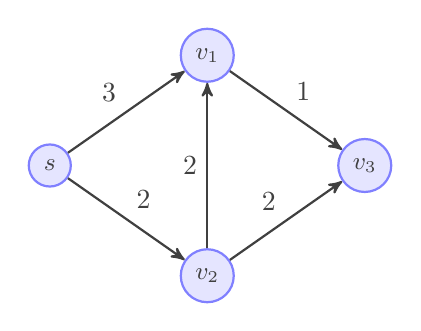
\begin{tikzpicture}[aaaa/.style={circle,draw=blue!50,fill=blue!10},thick,scale=2,
    gray!50!black,->,>=stealth']
    \node[aaaa] (v3) at (2, 1) {\small $v_3$};
    \node[aaaa] (v1) at (1, 1.7) {\small $v_1$}
    edge node[auto] {$1$} (v3);
    \node[aaaa] (v2) at (1, 0.3) {\small $v_2$}
    edge node[auto] {$2$} (v1)
    edge node[auto] {$2$} (v3);
    \node[aaaa] (s) at (0, 1) {\small $s$}
    edge node[auto] {$3$} (v1)
    edge node[auto] {$2$} (v2);
    \end{tikzpicture}
    \end{column}
    \end{columns}
\end{frame}

\begin{frame}{Weighted Bipartite Graph}
\begin{columns}[T]
\begin{column}{0.48\linewidth}
\begin{itemize}
    \item $n$ items and bidders.
    \item Each bidder has a value for each item.
    \item Assume this is a complete graph.
    \item Find the minimum cost bipartite matching.
    \vskip12pt
    \item These all give us greedy algorithms, but the
    idea is very general.
\end{itemize}
\end{column}
\begin{column}{0.48\linewidth}
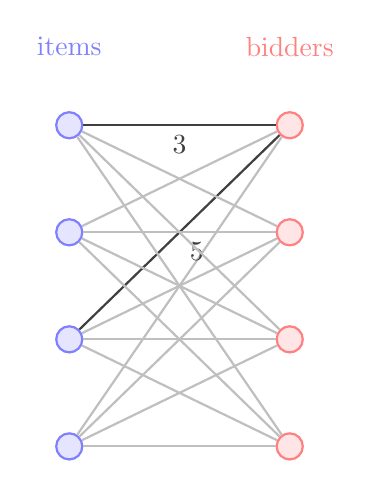
\begin{tikzpicture}[items/.style={circle,draw=blue!50,fill=blue!10},
bidders/.style={circle,draw=red!50,fill=red!10},thick,scale=2,gray!50!white]
\node[items] (i1) at (-0.7, 0) {};
\node[items] (i2) [below=of i1] {};
\node[items] (i3) [below=of i2] {};
\node[items] (i4) [below=of i3] {};
\node[bidders] (b1) at (0.7, 0) {}
edge (i2) edge (i4)
edge[gray!50!black] node[auto] {$3$} (i1)
edge[gray!50!black] node[auto] {$5$} (i3);
\node[bidders] (b2) [below=of b1] {}
edge (i1) edge (i2) edge (i3) edge (i4);
\node[bidders] (b3) [below=of b2] {}
edge (i1) edge (i2) edge (i3) edge (i4);
\node[bidders] (b4) [below=of b3] {}
edge (i1) edge (i2) edge (i3) edge (i4);
\node[blue!50] at (-0.7,0.5) {items};
\node[red!50] at (0.7,0.5) {bidders};
\end{tikzpicture}
\end{column}
\end{columns}
\end{frame}

\begin{frame}{Lattice-Linear Predicates (again)}
\begin{itemize}
    \item Definition (lattice-linear predicate). A predicate $B$ is
    \emph{lattice-linear} iff
    
    $$\forall G : \neg B(G) \implies \exists i : \mathrm{forbidden}(G, i).$$
    
    \item If $\neg B(G)$, then without advancing process $i$, it is
    impossible to make $B$ true.
\end{itemize}
    
\end{frame}

\begin{frame}{Efficient Advancement Property}
\begin{itemize}
    \item \emph{Efficient Advancement Property}: there exists
    an efficient (polynomial-time) function to determine the forbidden
    state.
    \item This holds for all our examples!
    \item Then there exists an algorithm to find some global state $G$
    that satisfies $B(G)$.
\end{itemize}
\end{frame}

\begin{frame}{Finding $G$ such that $B(G)$}
    \begin{framed}
var $G$ : array$[1, ..., N]$ of int, init $G[i] = \mathrm{initial}(i), \forall i$.
\vskip12pt

while $\neg B(G)$ do

\hskip12pt let $i$ be such that $\mathrm{forbidden}(G, i)$.
    
\hskip12pt if $(G[i] == \mathrm{final}(i))$, return false.
    
\hskip12pt else, $G[i] := \mathrm{next}(G[i])$.

end

return true and $G$.

    \end{framed}
\end{frame}

\begin{frame}{Lattice-Linear Predicates: more examples}
    
    \begin{itemize}
        \item Example: $B \equiv p_1 \textrm{ in CS } \wedge p_2 \textrm{ in CS }$
        is a conjunctive predicate, so it is lattice-linear!
        \item Example: ``$G$ is a consistent global state'' is lattice-linear.
        $G$ is not consistent if there is a send without its receive.
        So we must advance the process that needs to receive,
        otherwise there is no way for $G$ to be a CGS.
        \item We could actually advance multiple processes in parallel, if
        all are forbidden.
    \end{itemize}
    
\end{frame}

\begin{frame}{Regular Predicates}
\begin{columns}[T]
\begin{column}{0.48\linewidth}
\begin{itemize}
    \item Recall: $B$ lattice-linear $\Longleftrightarrow B$ closed under meets.
    \item $B$ is \emph{regular} if it is additionally closed under joins.
    \item That means that the set of consistent global states satisfying
    $B$ \emph{form a sublattice}.
\end{itemize}
\end{column}
\begin{column}{0.48\linewidth}
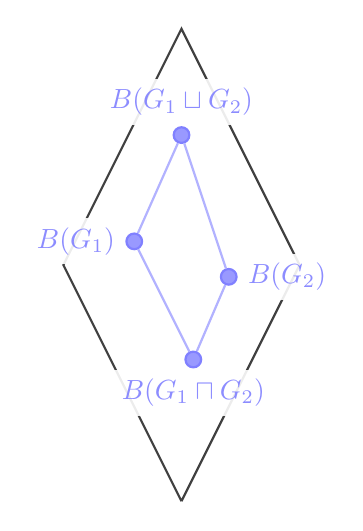
\begin{tikzpicture}[gray!50!black,thick,scale=1.5,
state/.style={draw=blue!50,fill=blue!40,circle,inner sep=2pt},
every label/.style={blue!50,fill=white,fill opacity=0.9},
every edge/.style={draw=blue!30}]
\draw (0,-2) -- (-1, 0) -- (0, 2) -- (1, 0) -- (0, -2);
\node[state] (g1) at (-0.4, 0.2) [label=left:$B(G_1)$] {};
\node[state] (g2) at (0.4, -0.1) [label=right:$B(G_2)$] {};
\node[state] (meet) at (0.1,-0.8) [label=below:$B(G_1 \sqcap G_2)$] {}
edge (g1) edge (g2);
\node[state] (join) at (0, 1.1) [label=above:$B(G_1 \sqcup G_2)$] {}
edge (g1) edge (g2);
\end{tikzpicture}
\end{column}
\end{columns}
\end{frame}

\begin{frame}{Regular Predicates: Examples}
\begin{itemize}
    \item Example. $B_1 \equiv $ there is no token message in transit.
    \item Example. $B_2 \equiv $ every request message has been acknowledged.
    \item Key property: if $B_1$ and $B_2$ are regular, then $B_1 \wedge B_2$
    is also regular.
    \item More examples: stable marriage, conjunctive predicates,
    weighted bipartite graph.
    \item The shortest path problem does \emph{not} satisfy regularity.
    \item For regular predicates, we could actually look at the lattice backwards
    if we wanted to.
\end{itemize}
    
\end{frame}

\begin{frame}{Closing remarks}
\begin{itemize}
    \item What is the minimum algorithm for detecting conjunctive
    predicates? (We will explore this in chapter 12.)
    \item A regular predicate is both linear (closed under meet) and
    post-linear (closed under join).
    \item Project proposals due this Thursday!
\end{itemize}
    
\end{frame}
\end{document}
